
\documentclass[12pt,a4paper,openany]{extarticle}
% подключаем собственный стилевой файл
\usepackage{mystyle}
\selectlanguage{russian}
\graphicspath{{./images/}}
\usepackage[pdftex]{lscape}
\usepackage{graphicx}
\usepackage{systeme}

\begin{document}
\part*{Лабораторная работа №4\\ Траекторное управление и задача планирования траектории.}
\section{Методические рекомендации}
\hspace*{\parindent}До начала работы студент должен выполнить предыдущие лабораторные этого цикла.

\section{Теоретические сведения}
\hspace*{\parindent}В прошлой работе вы успели ознакомиться с решением прямой и обратной задач кинематики для трехзвенного манипулятора. В данной лабораторной работе вам будет необходимо построить на основании знаний из второй лабораторной работы траекторный регулятор, способный следить за заданной траекторией с высокой точностью.
\paragraph*{Слежение за заданной траекторией}\\
Многозвенный манипулятор представляет из себя систему состоящую из \textit{n} сочленений. Каждое сочленение манипулятора испытывает момент нагрузки, обусловленный гравитационными силами, действующий на последующие сочленения и моменты сил вырабатываемые другими сочленениями, то есть каждое звено влияет на точность перемещения системы по заданной траектории. Следовательно слежение за траекторией можно разделить на две основных задачи. Во-первых, обеспечение слежения за траекторией путем регулирования напряжений в зависимости от информации полученной с датчиков. Во-вторых, компенсация создаваемых моментов сил и нагрузки.\\

В случае одномерного управления момент нагрузки рассматривается как внешний момент $M_l$.
Во второй лабораторной работе вы уже вывели передаточную функция от входа $M_u(s)$ к выходу $ \Theta(s)$ принимая $M_l(s)=0$:\\
\begin{equation}\label{eq:model}
frac{\Theta(s)}{M_u(s)}\approx \frac{1}{s(J_ms+K)},
\end{equation}
где $M_u(s) = \frac{K_m}{R}U(s)$, $K=K_f + \frac{K_eK_m}{R}$. Теперь получим передаточную функцию от входа $M_l(s)$ к выходу $ \Theta(s)$ принимая $U(s)=0$:\\
\begin{equation}\label{eq:model}
frac{\Theta(s)}{M_l(s)}\approx -\frac{1}{s(J_ms+K)},
\end{equation}

Комбинируя передаточные функции (1) и (2) получаем:\\
\begin{equation}\label{eq:model}
\Theta(s) = \frac{1}{s(J_ms + K)}(M_u(s)-M_l(s)) = P(s)(M_u(s) - M_l(s)),
\end{equation}

где \textit{P(s)} передаточная функция математической модели вращательного сочленения с учетом внешних моментов.\\

Первую задачу слежения за траекторией помогает решить ПИД-регулятор. Вы уже знакомы с ПИД-регулятором по скорости изображенном на рис. 4.1\\
\begin{center}
    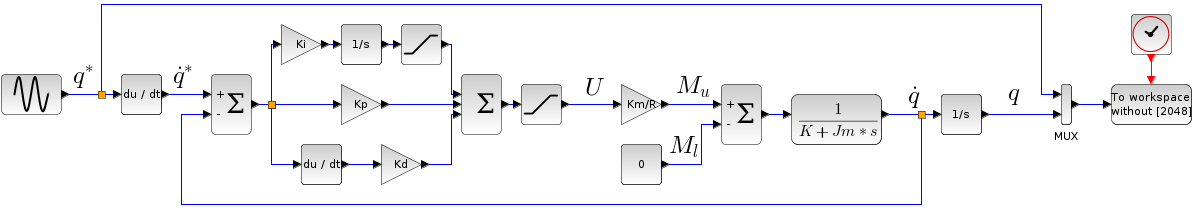
\includegraphics[width=\textwidth]{Lab4/images/Scheme_without.png}\\
    \centering{Рис 4.1 Система моделирования замкнутой системы с ПИД-регулятором}
\end{center}
\vspace{1cm}
 Как видно из ошибки моделирования слежения за траекторией представленной синусом, данной системе не хватает точности позиционирования, то есть манипулятор не точно отрабатывает траекторию.\\
 \vspace{1cm}
 \begin{center}
    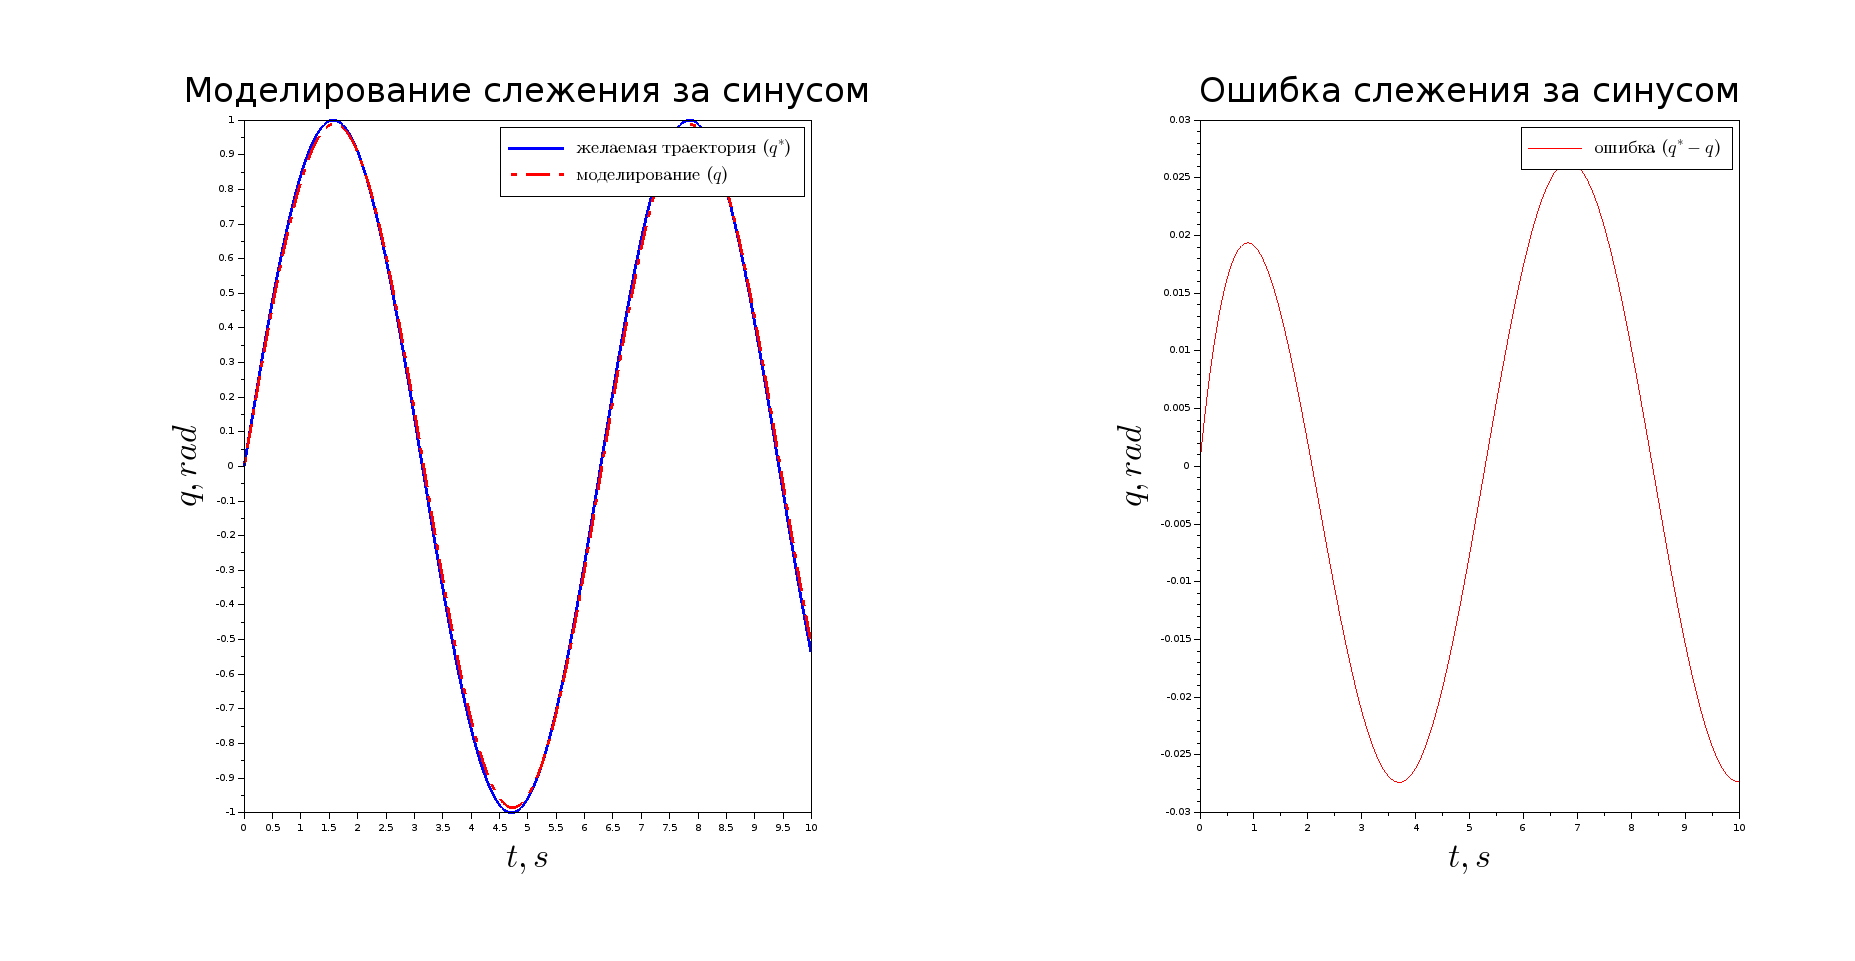
\includegraphics[width=0.8\textwidth]{Lab4/images/Pict_without.png}\\
    \centering{Рис 4.2 Моделирование слежения за синусом одного привода без внешнего воздействия}
\end{center}

\begin{center}
    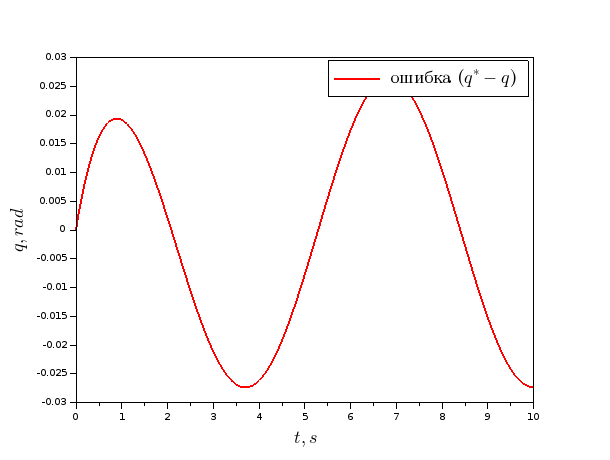
\includegraphics[width=0.8\textwidth]{Lab4/images/Error_without.png}\\
    \centering{Рис 4.3 Ошибка слежения за синусом одного привода без внешнего воздействия}
\end{center}
\vspace{1cm}
Для решения второй задачи слежения за траекторией необходимо сделать траекторный регулятор.Пропорционального регулятора по углу будет вполне достаточно. Реализацию данного регулятора можно найти в схеме моделирования представленной на рис. 4.4. \\
\vspace{1cm}
\begin{center}
    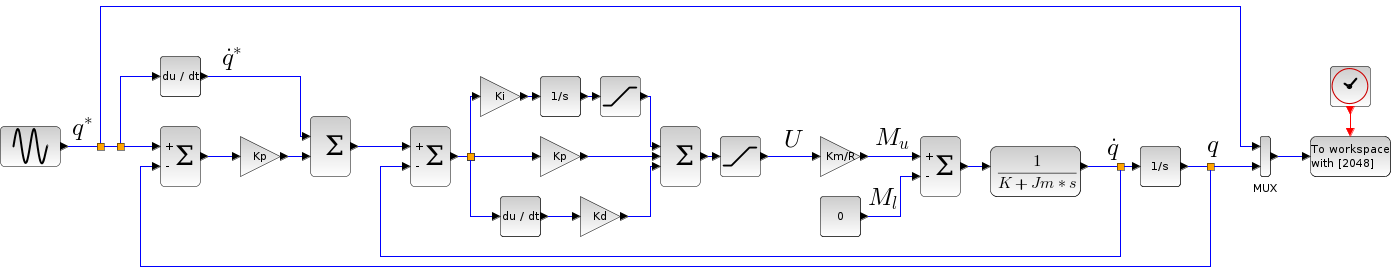
\includegraphics[width=\textwidth]{Lab4/images/Scheme_with.png}\\
    \centering{Рис 4.4 Система моделирования замкнутой системы с траекторным регулятором}
\end{center}
\begin{center}
Как можно заметить после внедрения траекторного регулятора сочленение стало лучше следовать за синусом и порядок ошибки уменьшился.
    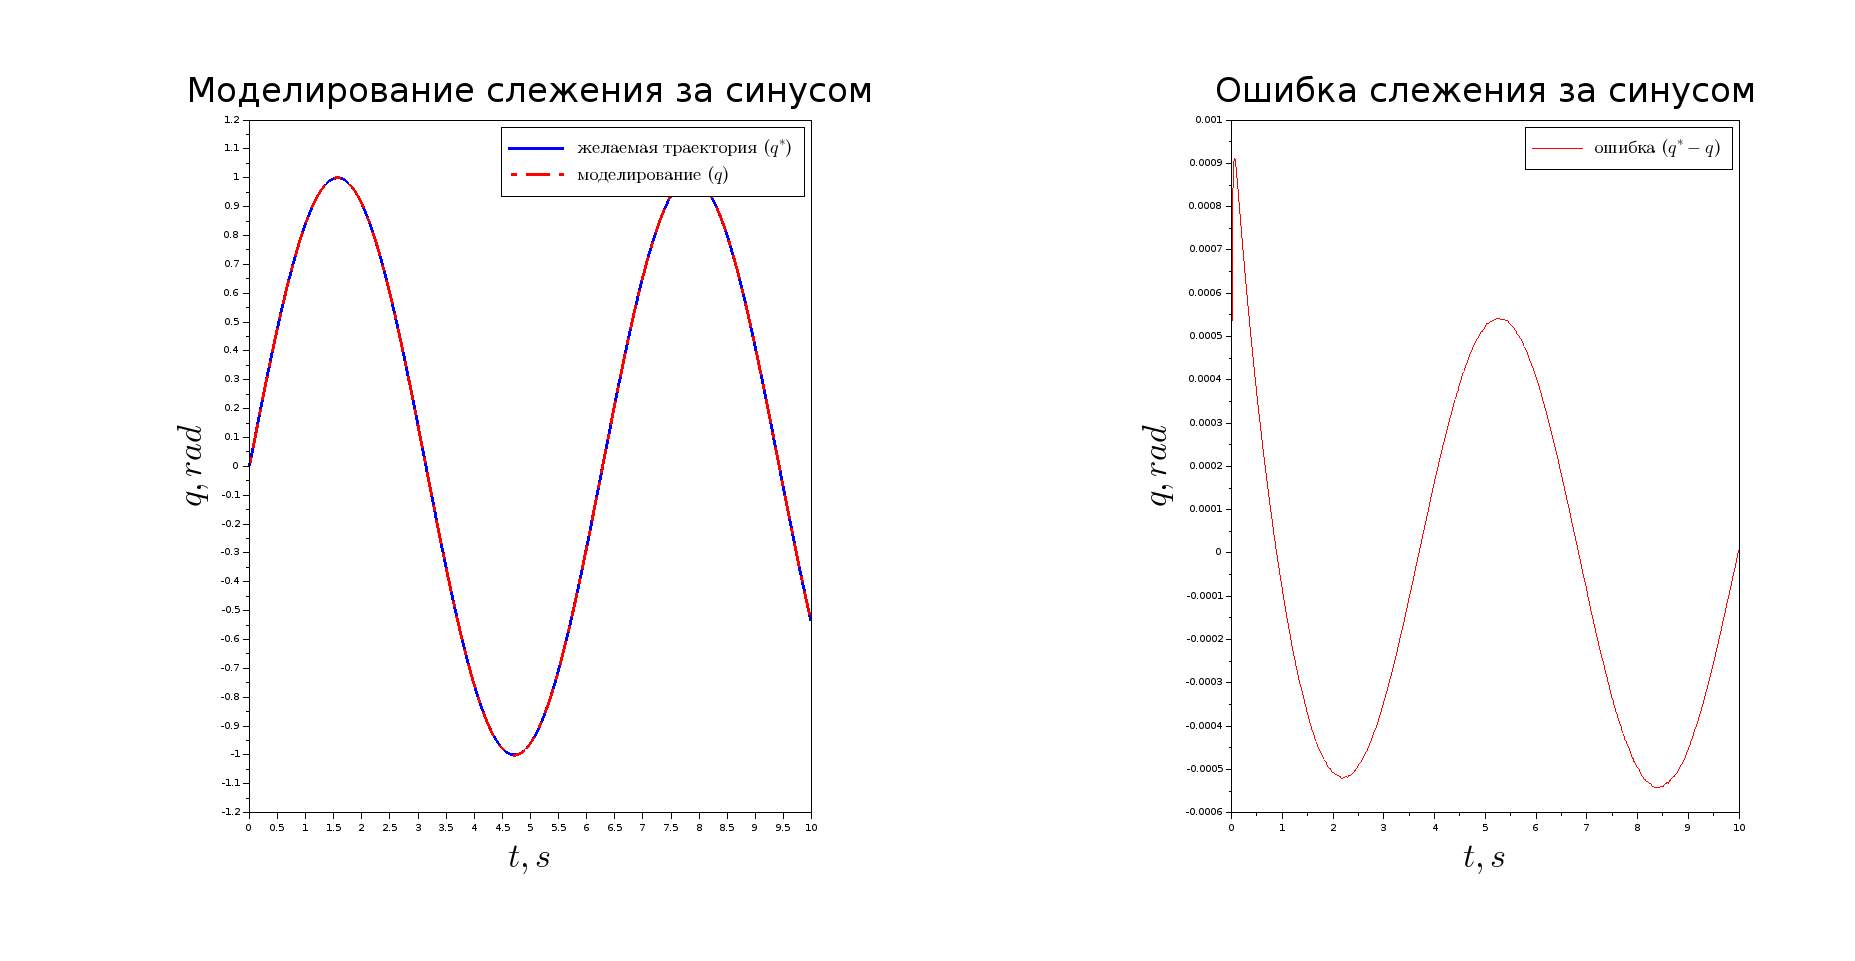
\includegraphics[width=0.8\textwidth]{Lab4/images/Pict_with.png}\\
    \centering{Рис 4.5 Моделирование слежения за синусом одного привода с траекторным регулятором}
\end{center}

\begin{center}
    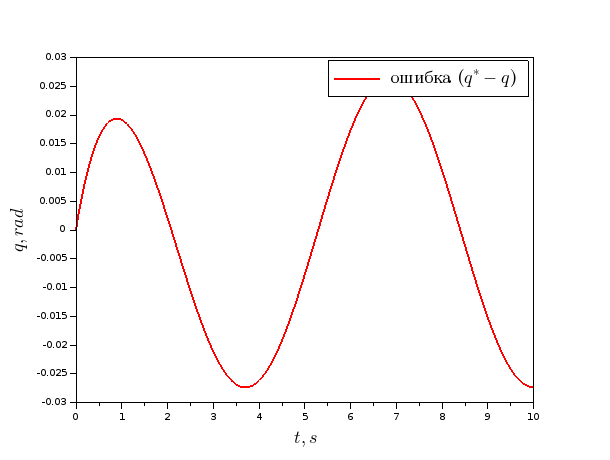
\includegraphics[width=0.8\textwidth]{Lab4/images/Error_without.png}\\
    \centering{Рис 4.6 Ошибка слежения за синусом одного привода с траекторным}
\end{center}
\newpage
Чтобы наглядно показать влияние траекторного регулятора на точность следования желаемой траектории на рисунке 4.7 приведен график сравнения двух ошибок.
\begin{center}
    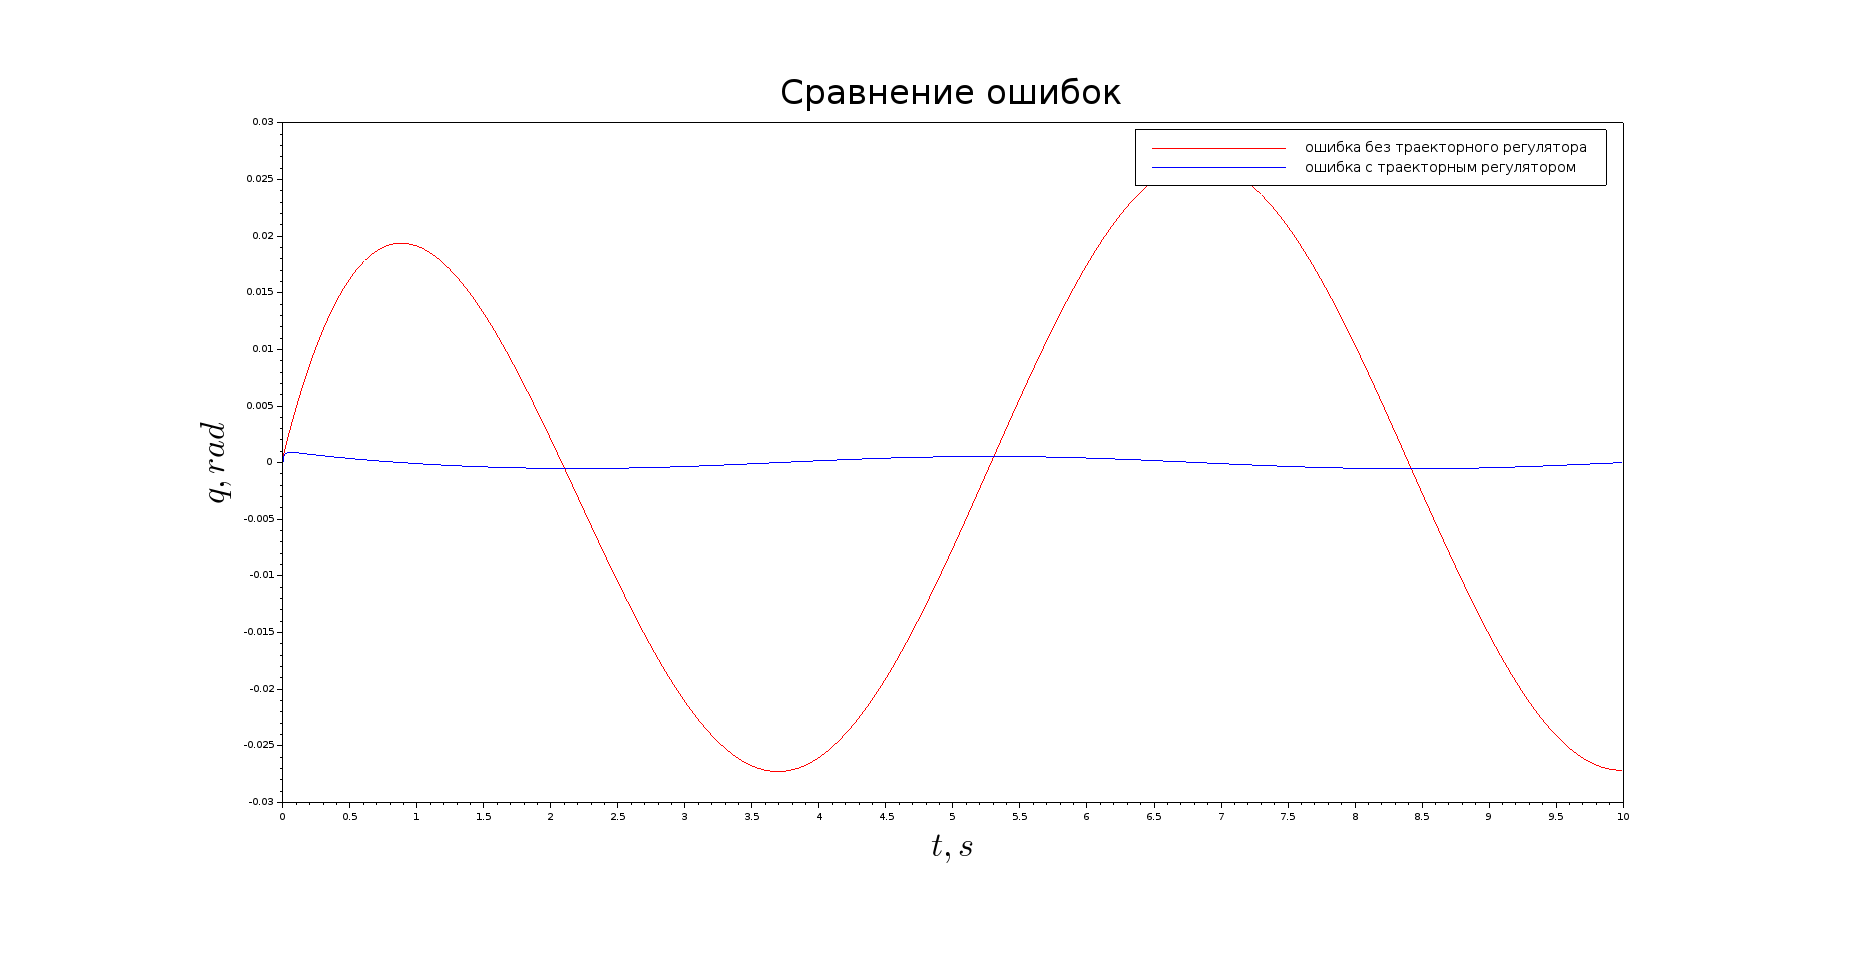
\includegraphics[width=0.8\textwidth]{Lab4/images/Error_comparison.png}\\
    \centering{Рис 4.7 Система моделирования замкнутой системы с ПИД-регулятором}
\end{center} %Импорт Диминой части
\paragraph*{Планировщик траектории}$\phantom{-}$\\
\hspace*{\parindent} Основной задачей планирования траектории является поиск непрерывного закона движения манипулятора, а именно параметризация пути временем:
\begin{equation}\label{eq:model}
    \begin{bmatrix}
    q_{1} \\
    q_{2} \\
    q_{3} \\
    \end{bmatrix}
    =
     \begin{bmatrix}
    q_{1}(t) \\
    q_{2}(t) \\
    q_{3}(t) \\
    \end{bmatrix}
\end{equation} 
Закон движения нужен в первую очередь, чтобы звенья манипулятора двигались согласованно, то есть в начальный и конечный момент времени все звенья начинали и заканчивали свое движение одновременно.
При этом для планирования траектории необходимо знать динамические ограничения системы, а именно максимальную скорость и ускорение выходных валов редукторов в сочленениях: $q_{i_{max}}$ и $\dot{q}_{i_{max}}$\\
Рассмотрим задачу перемещения манипулятора из одной конфигурации в (Point to Point). При этом известны только граничные значения обобщенных координат и скоростей: $q_s=q(0)$, $\dot{q}_s=\dot{q}(t_0)$, $q_f=q(t_f)$, $\dot{q}_f=\dot{q}(t_f)$, где $t_0$ $t_f$ - начальное и конечное время соответственно. Необходимо найти значение обобщенных координат манипулятора в каждый момент времени $t\in [t_0, t_f]$.
\begin{center}
    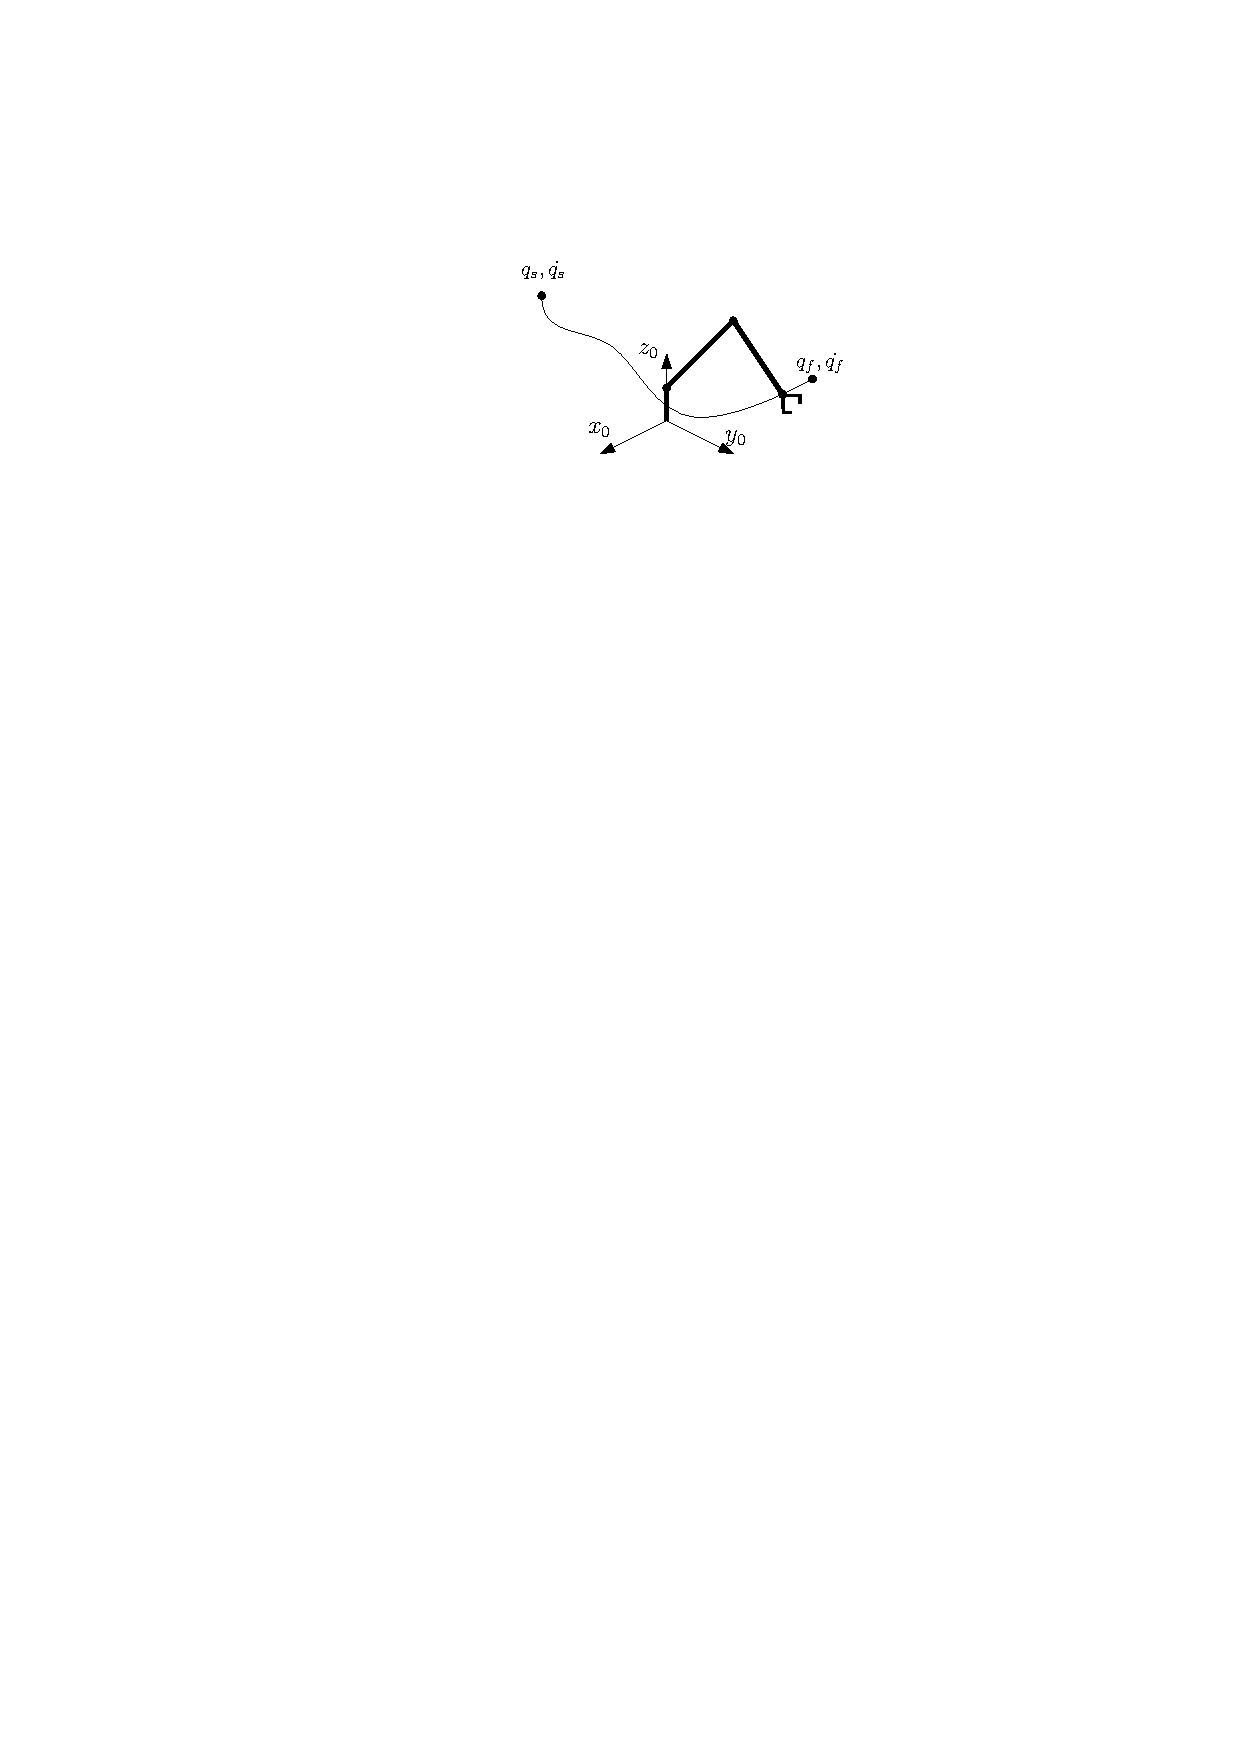
\includegraphics[width=0.45\textwidth]{Lab4/images/trjPlanningbetweenPoint.pdf}\\
    \centering{Рис 1.1 Граничные условия для планирования траектории.}
\end{center}

\paragraph*{Сплайн интерполяция}$\phantom{-}$\\

Одним из самых распространенных подходов планирования траектории является сплайн-интерполяция. Рассмотрим основную идею процесса интерполяции сплайном с точки зрения лин. алгебры. В рамках нашей задачи ограничимся интерполяцией сплайном третьей степени, ввиду зашумленности измерения ускорений двигателя и как следствие невозможности управления ими. В таком случае уравнение движения для каждого звена манипулятора $q_i(t)$ задается следующим образом:
\begin{equation}\label{eq:model}
q_i(t)=a_{i,1}\cdot t^3  + a_{i,2}\cdot t^2 + a_{i,3}\cdot t + a_{i,4}
\end{equation}
, где $a_{i,1}, a_{i,2}, a_{i,3}, a_{i,4}$ - неизвестные коэффициенты полинома.
Продифференцируем его для получения угловых скоростей и получим:
\begin{equation}\label{eq:model}
\dot{q}_i(t)=3a_{i,1}\cdot t^2  + 2a_{i,2}\cdot t + a_{i,3}
\end{equation}


\begin{center}
    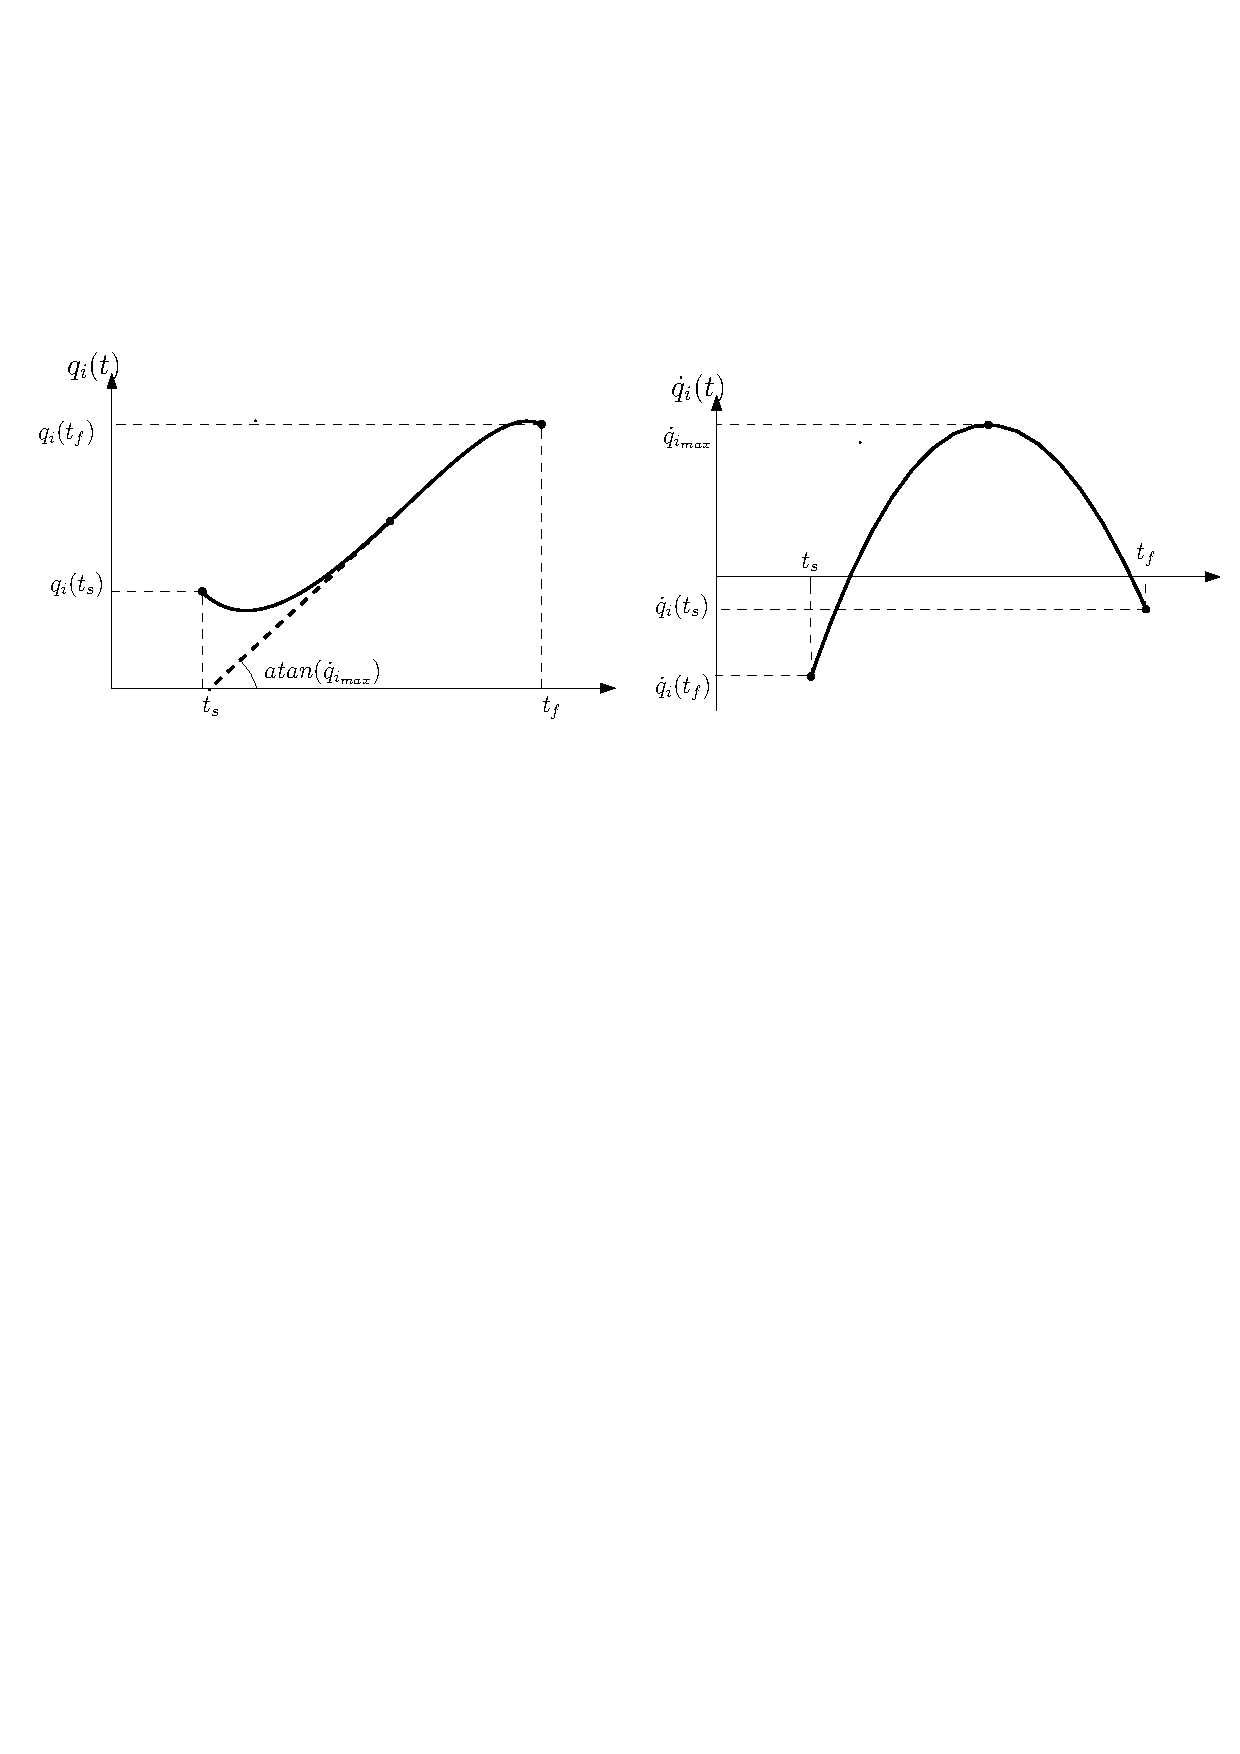
\includegraphics[width=\textwidth]{Lab4/images/cubicTrjPlanning.pdf}\\
    \centering{Рис 1.2 Интерполяция кубическим сплайном.}
\end{center}

Теперь вспомним о том, что нам известны начальные и конечные значения обобщенных координат и скоростей: $q_{i_{s}}, q_{i_{f}},\dot{q}_{i_{s}}, \dot{q}_{i_{f}}$, а также времени $t_s$ и $t_f$ подставив их в уравнения сформируем систему:
\begin{equation}\label{eq:model}
\systeme*{
q_{i_{s}}=a_{i,1}\cdot t_s^3  + a_{i,2}\cdot t_s^2 + a_{i,3}\cdot t_s + a_{i,4},
q_{i_{f}}=a_{i,1}\cdot t_f^3  + a_{i,2}\cdot t_f^2 + a_{i,3}\cdot t_f + a_{i,4},
\dot{q}_{i_{s}}=3a_{i,1}\cdot t_s^2  + 2a_{i,2}\cdot t_s + a_{i,3},
\dot{q}_{i_{f}}=3a_{i,1}\cdot t_f^2  + 2a_{i,2}\cdot t_f + a_{i,3}
}
\end{equation}
Теперь перейдем непосредственно к интерполяции. Чтобы найти закон движения (1) для каждого звена необходимо определить коэффициенты $a_{i,1}, a_{i,2}, a_{i,3}, a_{i,4}$. Как видно из уравнений выше, если принять в них эти коэффициенты как неизвестные параметры, то получится так, что мы имеем \textbf{4 уравнения и 4 неизвестных параметра}.
Таким образом, мы однозначно сможем разрешить систему уравнений относительно параметров $a_{i,1}, a_{i,2}, a_{i,3}, a_{i,4}$.
Воспользуемся для этого матричным представлением системы линейных алгебраических уравнений:
\begin{equation}\label{eq:model}
     \begin{bmatrix}
    q_{i_{s}} \\
    q_{i_{f}} \\
    \dot{q}_{i_{s}} \\
    \dot{q}_{i_{f}} \\
    \end{bmatrix}
    =
    \begin{bmatrix}
    t^3_s & t^2_s & t_s & 1\\
    t^3_f & t^2_f & t_f & 1\\
    3t^2_s & 2t_s & 1 & 0\\
    3t^2_f & 2t_f & 1 & 0\\
    \end{bmatrix}
    \begin{bmatrix}
    a_{i,1}\\
    a_{i,2}\\
    a_{i,3}\\
    a_{i,4}\\
    \end{bmatrix}
\end{equation}
Перепишем данное выражение в удобном для представления виде:
\begin{equation}\label{eq:model}
b_i = M_i a_i
\end{equation}
, где $M$ - матрица коэффициентов, $a_i=[a_{i,1}, a_{i,2}, a_{i,3}, a_{i,4}]^T$ - вектор искомых параметров,  $b_i=[q_{i_{s}}, q_{i_{f}}, \dot{q}_{i_{s}}, \dot{q}_{i_{f}}]^T$ - вектор граничных условий.
Теперь можно найти вектор параметров $a_i$, обратив матрицу $M_i$:
\begin{equation}\label{eq:model}
a_i = M_i^{-1} b_i 
\end{equation}
Вернемся снова к уравнению движения отдельного звена манипулятора (2) и подставим теперь уже известные из выражения (7) коэффициенты $a_i=[a_{i,1}, a_{i,2}, a_{i,3}, a_{i,4}]$:
\begin{equation}\label{eq:model}
q_i(t)=
    \begin{bmatrix}
    a_{i,1} & a_{i,2} & a_{i,3} & a_{i,4}
    \end{bmatrix}
    \begin{bmatrix}
    t^3\\
    t^2\\
    t\\
    1\\
    \end{bmatrix}
\end{equation}
Данное выражение можно определить для оставшихся звеньев манипулятора при тех же $t_f$,$t_s$ и соответствующих $q_{i_{s}}$,$q_{i_{f}}$.
В итоге уравнение движения трехзвенного манипулятора будет записано в следующем виде:
\begin{equation}\label{eq:model}
\begin{bmatrix}
    q_1(t)\\
    q_2(t)\\
    q_3(t)\\
\end{bmatrix}
    =
\begin{bmatrix}
    a_{1,1} & a_{1,2} & a_{1,3} & a_{1,4}\\
    a_{2,1} & a_{2,2} & a_{2,3} & a_{2,4}\\
    a_{3,1} & a_{3,2} & a_{3,3} & a_{3,4}\\
\end{bmatrix}
\begin{bmatrix}
    t^3\\
    t^2\\
    t\\
    1\\
    \end{bmatrix}
\end{equation}

Стоит отметить, что выбирая $\Delta t=t_f - t_s$ нужно учесть $\dot{q}_{i_{max}}$ и $\ddot{q}_{i_{max}}$

\paragraph*{Метод линейных сегментов с параболическими частями(LSPB)}$\phantom{-}$\\

Другим наиболее распространенным способом генерации траектории является метод линейных сегментов с параболическими частями. В английской литературе данный метод можно встретить под названием  "Linear segments with parabolic blends". В большинстве случаев этот метод применяется, когда необходимо двигаться от точки до точки, останавляваясь в них.\\

Уравнение движения для данного метода состоит из трех частей:\\ 1)равноускоренное движение ($\ddot{q_i}=const,\ddot{q_i}>0$).\\
2)равномерное движение($\dot{q_i}=const$).\\
3)равнозамедленное движение($\ddot{q_i}=const,\ddot{q_i}<0$).\\

\begin{center}
    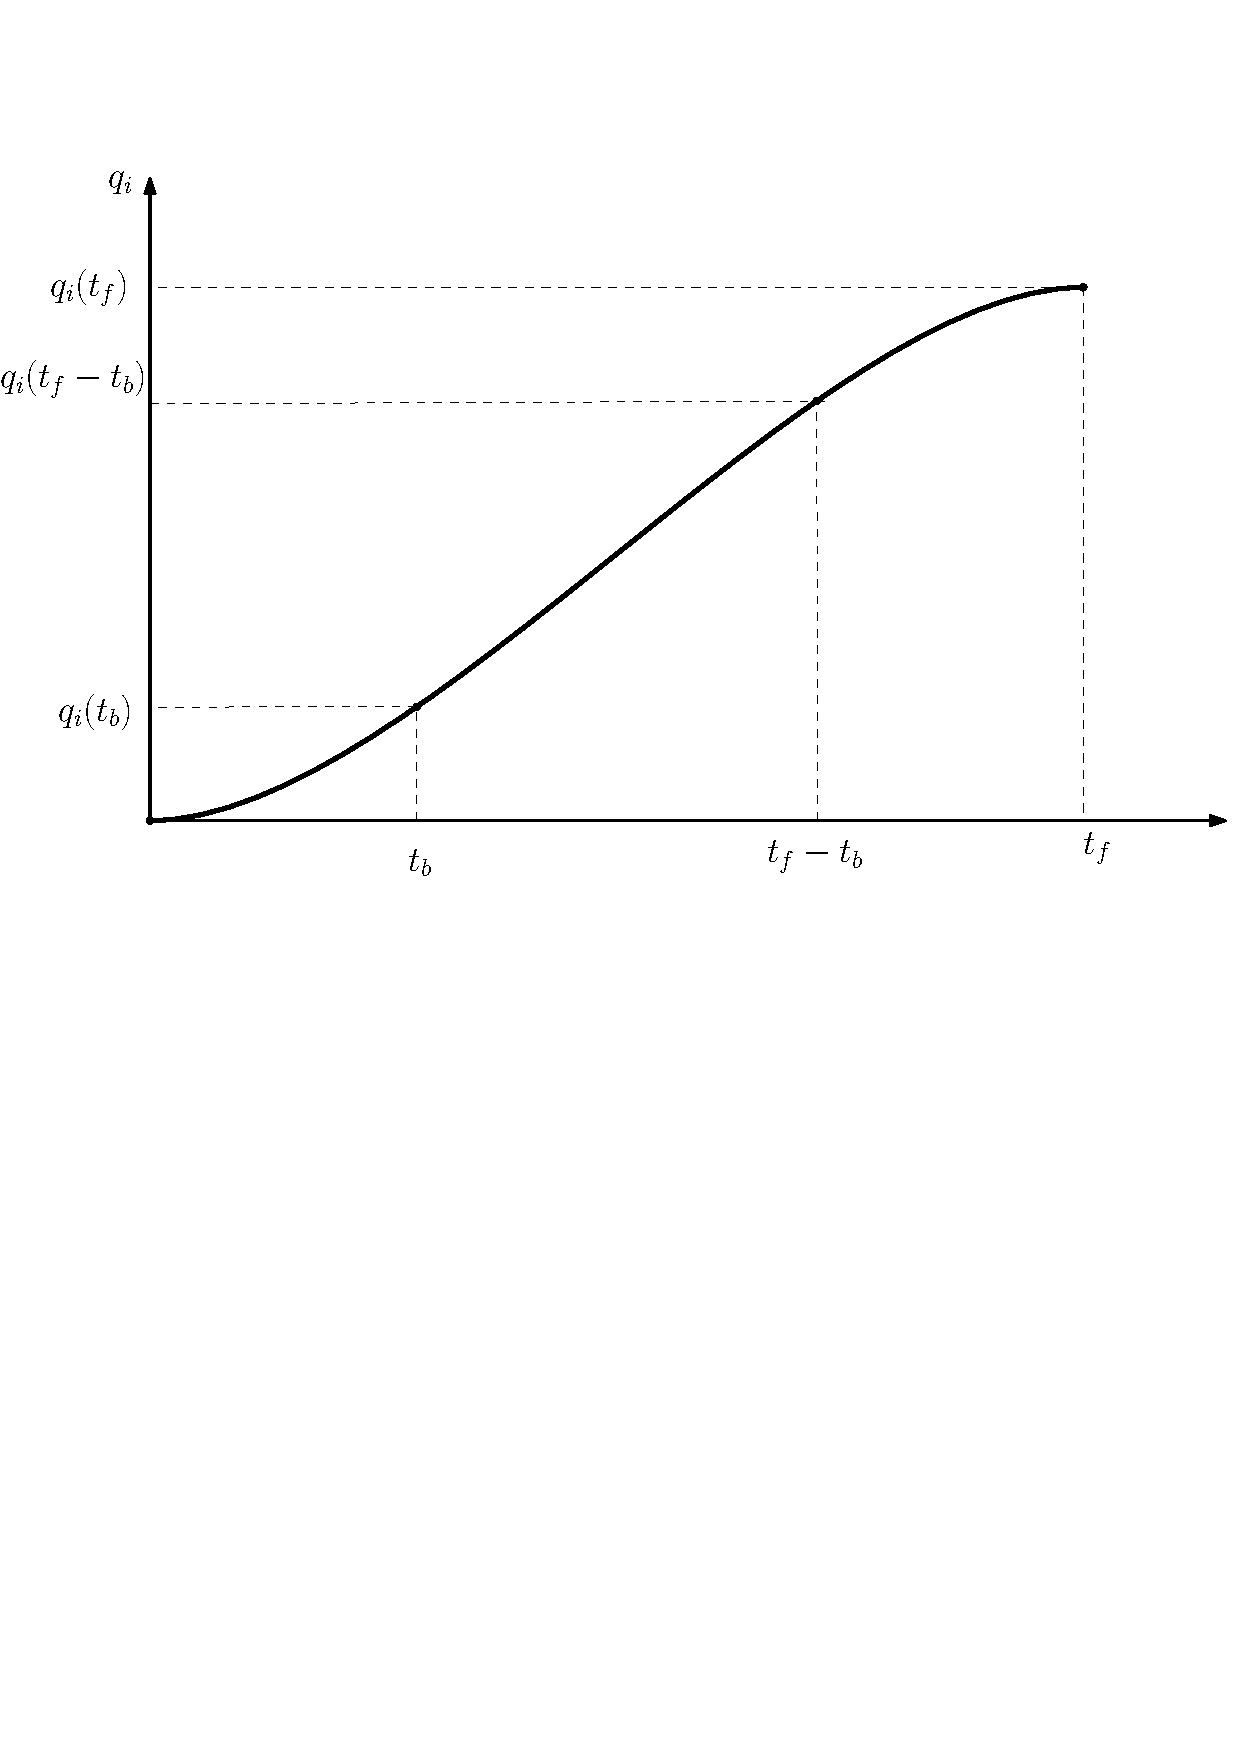
\includegraphics[width=0.8\textwidth]{Lab4/images/LSPB.pdf}\\
    \centering{Рис 1.3 Граничные условия для планирования траектории.}
\end{center}

Первая часть представляет из себя процесс разгона привода до некоторой постоянной скорости, обозначим ее как $V_i$.
Из курса физики вам известно, что движение c постоянным ускорением $A$ имеет следующий закон: 
$$
    \ddot{q}_i=const
$$
$$
    \dot{q}_i=c_{i,2}\cdot t+c_{i,1}
$$
$$
    q_i=c_{i,2}\cdot t^2+c_{i,1}\cdot t+c_{i,0}
$$

, где $c_{i,0}, c_{i,1}, c_{,2}$ -неизвестные константы, причем $c_{i,0}=q_i(t_s)$,$ c_{i,1}=\dot{q}(t_s)$,$ c_{i,2}=A$
Для того, чтобы найти эти коэффициенты,  необходимо вспомнить о том, что в рамках нашей задачи в начальный момент времени скорость движения звена $\dot{q}_i(t_s)=0$, тогда $c_{i,1}=0$.\\

Обозначим время в течении которого звено двигается с ускорением $A$, как $t_b$. В таком случае $\dot{q}_i(t_b)=c_{i,2}\cdot t_b+c_{i,1} = V$, это и есть та постоянная скорость с которой будет происходить движение пока $t\in[t_b,t_f-t_b]$.


 
\end{document}